%!TeX root=MemoriaTFG.tex

\section{Bloc 1: línia base i \emph{curriculum learning}}
\label{sec:bloc1}

El primer bloc estableix un punt de partida rigorós (Fase~1) i introdueix la primera
tècnica que trenca el sostre de rendiment inicial (Fase~2, \emph{curriculum learning}).
El Checkpoint~1 tanca el bloc seleccionant els dos models que continuen.

\subsection{Fase 1: comparativa homogènia d'algorismes}
\label{sec:fase1}

\paragraph{Hipòtesi.} Abans d'aplicar cap tècnica avançada cal saber quin algorisme
parteix amb avantatge. La Fase~1 compara quatre algorismes d'\ac{AR} en igualtat de
condicions i partint de zero, sense cap coneixement previ del joc.

\paragraph{Disseny.} Es comparen quatre agents que cobreixen les dues grans famílies
d'algorismes d'\ac{AR}: els \textbf{basats en la funció de valor} (com el DQN, que aprèn
quant val cada acció i n'extreu la política) i els \textbf{basats en el gradient de la
política} (com el PPO, que optimitza directament la política). Es reparteixen també entre
les variants \emph{on-policy} i \emph{off-policy} (definides al capítol~\ref{cap:marc}) i
entre les dues biblioteques emprades (taula~\ref{tab:fase1-algorismes}). Tots comparteixen
la mateixa observació de
240~dimensions, la mateixa arquitectura \ac{MLP} de \([256, 256]\) sense extractor
convolucional, i la mateixa funció d'avaluació; així qualsevol diferència s'atribueix a
l'algorisme i no a l'arquitectura.

\begin{table}[H]
  \centering
  \begin{tabular}{llll}
    \toprule
    Algorisme & Biblioteca & Política & Paral·lelisme \\
    \midrule
    DQN-RLCard  & RLCard & Off-policy        & 1 entorn seqüencial \\
    NFSP-RLCard & RLCard & Off-policy + \acs{SL} & 1 entorn seqüencial \\
    DQN-SB3     & \ac{SB3} & Off-policy      & 1 entorn \\
    PPO-SB3     & \ac{SB3} & On-policy       & 48 entorns (\emph{SubprocVecEnv}) \\
    \bottomrule
  \end{tabular}
  \caption{Els quatre algorismes comparats a la Fase~1.}
  \label{tab:fase1-algorismes}
\end{table}

\emph{Avaluació en dues òptiques.} Com que els algorismes tenen velocitats molt
diferents, comparar-los només per passos seria injust amb els paral·lelitzables. Per això
es mesura el rendiment sota dues òptiques complementàries:
\begin{itemize}
  \item \textbf{Per passos} (5~milions): la qualitat assolida després del mateix nombre de
        passos d'entrenament (eficiència per mostra).
  \item \textbf{Per temps real} (4~hores per agent): la qualitat assolida amb el mateix
        pressupost temporal (rendiment efectiu segons el \emph{throughput}).
\end{itemize}

\emph{Oponents.} Cada agent s'entrena contra una barreja d'oponents
(taula~\ref{tab:fase1-oponents}) amb un criteri comú: una petita fracció de
l'agent aleatori (per mantenir diversitat i explorar estats poc habituals) i un gruix
de l'agent basat en regles (el senyal estratègic principal). La diferència és el
\emph{self-play}: els agents de RLCard (DQN i NFSP) el suporten de manera nativa, de manera
que un 30\% de les partides es juguen contra una versió del propi agent. En el cas del DQN,
aquesta versió és una còpia \emph{Polyak} que s'actualitza lentament (un 5\% cap als pesos  
actuals cada 5\,000~passos): així l'oponent millora amb l'agent però no canvia tan de
pressa com per desestabilitzar l'aprenentatge.

\begin{table}[H]
  \centering
  \begin{tabular}{lccc}
    \toprule
    Agent & Random & l'agent basat en regles & Self-play \\
    \midrule
    DQN-RLCard  & 10\%      & 60\%       & 30\% (Polyak) \\
    NFSP-RLCard & 10\%      & 60\%       & 30\% (natiu) \\
    DQN-SB3     & 5\%       & 95\%       & — \\
    PPO-SB3     & 5\%       & 95\%       & — \\
    \bottomrule
  \end{tabular}
  \caption{Distribució d'oponents per episodi a la Fase~1. Els agents de RLCard
           incorporen self-play; els de \ac{SB3} entrenen només contra oponents fixos
           (l'agent aleatori i l'agent basat en regles), sense self-play.}
  \label{tab:fase1-oponents}
\end{table}

\emph{Bucle d'entrenament.} Els dos agents de RLCard s'entrenen
amb un bucle manual: controla el
format de cada transició que s'injecta al \emph{replay buffer}, alterna la posició de
l'aprenent a cada partida i resol l'assignació de crèdit quan és l'oponent qui tanca la
partida (la recompensa terminal s'assigna a la darrera jugada de l'aprenent). Els agents
\ac{SB3} usen la rutina nativa de la biblioteca amb un \emph{callback} que avalua i desa el
millor model cada 500\,000~passos. PPO genera l'experiència amb 48~entorns en paral·lel
repartits entre oponents i posicions. Per garantir que l'avaluació mesura generalització i
no memorització, l'agent basat en regles de l'avaluació s'instancia amb una llavor diferent
de la d'entrenament.

\paragraph{Resultats.} Cap agent assoleix un rendiment alt \emph{i} estable alhora
(taula~\ref{tab:fase1-resultats}). DQN-SB3 és el millor en totes dues òptiques (pic del
62{,}8\% per passos i 58{,}5\% per temps), però pateix una degradació severa cap al final
de l'entrenament (de 62{,}8\% a 36{,}5\%): la seva millor mètrica és molt superior a la
final. PPO-SB3 és el més feble a igualtat de passos (29{,}5\%), perquè un algorisme
on-policy necessita molts més passos per estabilitzar-se, però té un \emph{throughput}
incomparable (taula~\ref{tab:fase1-throughput}): genera 36{,}5~milions de passos per hora,
28~vegades més que NFSP. Aquest contrast fa que el rànquing canviï entre les dues òptiques.
El patró comú a tots els agents és la \textbf{inestabilitat}: regredeixen cap al final de
l'entrenament, senyal que el problema (partida llarga, recompensa molt diferida) no
proporciona un senyal d'aprenentatge prou estable.

\begin{table}[H]
  \centering
  \begin{tabular}{lcccc}
    \toprule
    & \multicolumn{2}{c}{Per passos (5M)} & \multicolumn{2}{c}{Per temps (4~h)} \\
    \cmidrule(lr){2-3}\cmidrule(lr){4-5}
    Agent & Millor & Final & Millor & Final \\
    \midrule
    DQN-SB3     & \textbf{62{,}8\%} & 36{,}5\% & \textbf{58{,}5\%} & 17{,}2\% \\
    NFSP-RLCard & 53{,}2\% & 29{,}0\% & 43{,}0\% & 33{,}2\% \\
    DQN-RLCard  & 51{,}0\% & 25{,}8\% & 44{,}5\% & 34{,}2\% \\
    PPO-SB3     & 29{,}5\% & 18{,}5\% & 42{,}0\% & 21{,}2\% \\
    \bottomrule
  \end{tabular}
  \caption{\texttt{metric} de la Fase~1 sota les dues òptiques. «Millor» és el pic durant
           l'entrenament; «Final» és el valor en acabar, que evidencia la inestabilitat.}
  \label{tab:fase1-resultats}
\end{table}

\begin{table}[H]
  \centering
  \begin{tabular}{lrr}
    \toprule
    Algorisme & Passos/hora & Factor vs NFSP \\
    \midrule
    PPO-SB3     & 36{,}5\,M & 28$\times$ \\
    DQN-SB3     & 7{,}0\,M  & 5{,}4$\times$ \\
    DQN-RLCard  & 5{,}5\,M  & 4{,}2$\times$ \\
    NFSP-RLCard & 1{,}3\,M  & 1$\times$ \\
    \bottomrule
  \end{tabular}
  \caption{\emph{Throughput} dels quatre algorismes. El paral·lelisme de PPO-SB3 el fa
           28~vegades més ràpid que NFSP-RLCard.}
  \label{tab:fase1-throughput}
\end{table}

\begin{figure}[H]
  \centering
  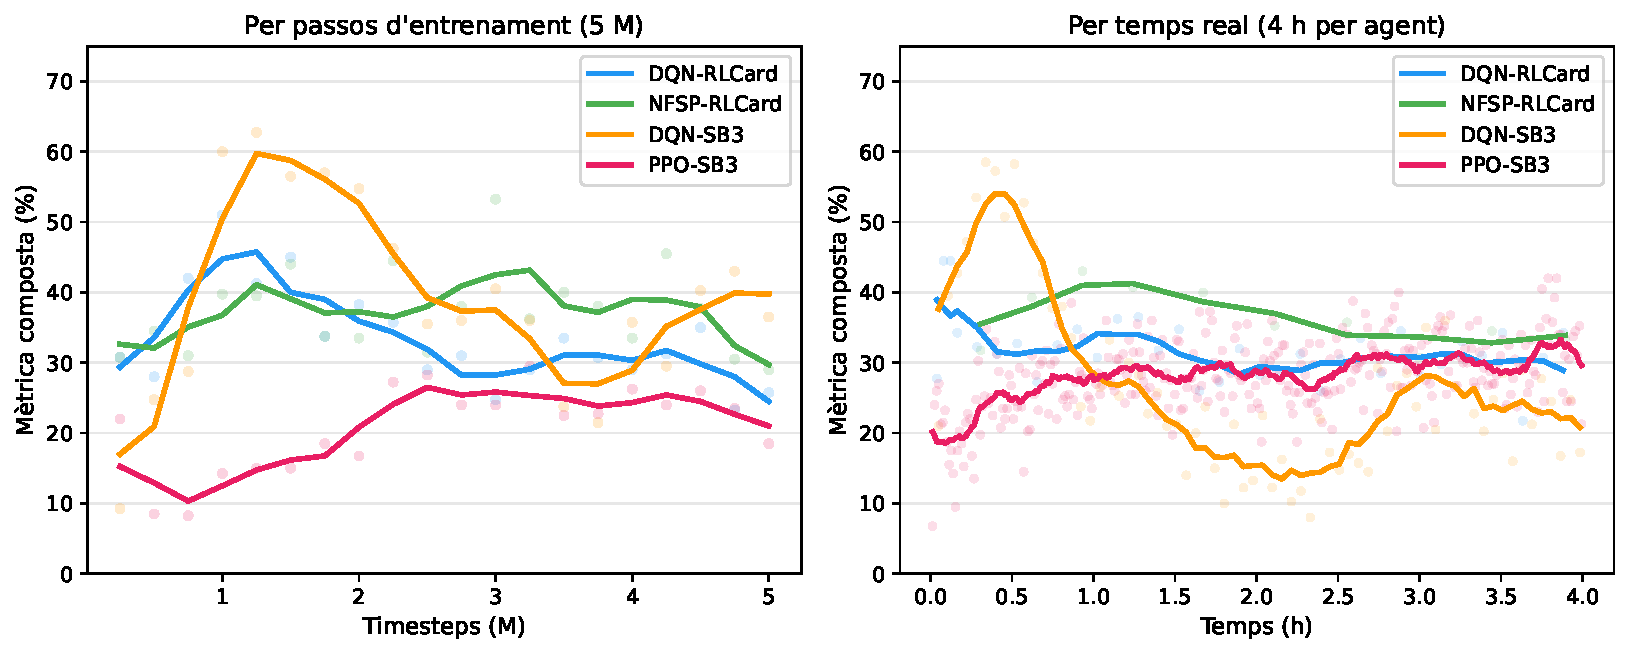
\includegraphics[width=\textwidth]{figures/fase1/corbes_ts.pdf}
  \caption{Mètrica composta de la Fase~1 sota les dues òptiques d'avaluació.
           A l'esquerra, rendiment als 5~M passos d'entrenament (eficiència per
           mostra); a la dreta, rendiment al llarg de 4~hores de còmput per agent
           (rendiment efectiu). DQN-SB3 lidera en ambdues, però el rànquing
           de la resta canvia: PPO-SB3 és el pitjor per passos però supera
           DQN-RLCard i NFSP-RLCard per temps gràcies al seu \emph{throughput}.}
  \label{fig:fase1-corbes-ts}
\end{figure}

\paragraph{Decisió.} El coll d'ampolla no és el còmput sinó el \textbf{senyal
d'aprenentatge}. El cas més clar és PPO-SB3: és l'agent més escalable i ràpid, però el que
menys aprofita una partida llarga amb recompensa diferida. La hipòtesi que en sorgeix és
que factoritzar la partida en unitats més curtes i denses (mans) hauria de donar un senyal
molt més ric. Això motiva la Fase~2.

\emph{Nota sobre l'observació.} Les Fases~1 i~2 van utilitzar una versió primerenca del
vector de context de 23~dimensions (239~dimensions en total). A partir de la Fase~3 es va
ampliar a 24~dimensions (240 en total), tal com es descriu al capítol~\ref{cap:entorns}.
El canvi no afecta les conclusions comparatives, atès que totes les sèries d'una mateixa
fase comparteixen la mateixa observació.

\subsection{Fase 2: \emph{curriculum learning} (mà $\rightarrow$ partida)}
\label{sec:fase2}

\paragraph{Hipòtesi.} Entrenar directament sobre partides senceres obliga l'agent a
resoldre alhora dos problemes acoblats: jugar bé cada mà (tàctica local) i gestionar el
marcador al llarg de la partida (estratègia global). El \emph{curriculum
learning}~\cite{bengio2009curriculum}, que presenta primer els exemples simples i després
els complexos, permet desacoblar-los. Al Truc, una \emph{mà} és la unitat natural simple:
episodi curt ($\sim$15~passos) i recompensa calculable al final. La hipòtesi és que
entrenar primer sobre mans (amb l'entorn \texttt{TrucEnvMa} descrit al
capítol~\ref{cap:entorns}) i després fer \emph{finetune} sobre partides senceres accelera i
millora l'aprenentatge respecte a entrenar-hi directament.

\paragraph{Disseny.}

\emph{El curriculum de dues etapes.} S'ha dissenyat un curriculum que va de la tasca densa
i curta a l'escassa i llarga (figura~\ref{fig:fase2-curriculum}):
\begin{enumerate}
  \item \textbf{Etapa de mans} (12M passos): l'agent s'entrena a \texttt{TrucEnvMa}, on
        cada mà és un episodi independent ($\sim$15~passos) amb recompensa densa
        normalitzada ($\text{punts}/24$). Aquí aprèn la tàctica local: quan jugar fort,
        quan acceptar un envit, quan plantar el truc.
  \item \textbf{Etapa de partides} (12M passos): els pesos apresos es transfereixen a
        \texttt{TrucEnv}, on l'episodi és una partida sencera fins a 24~punts. L'agent
        parteix d'una política ja formada i el \emph{finetune} recau sobre l'estratègia a
        llarg termini, com la gestió del marcador.
\end{enumerate}

\begin{figure}[H]
  \centering
  \begin{tikzpicture}[
      box/.style={draw, rounded corners=3pt, minimum width=3.6cm, minimum height=1.5cm,
                  align=center, font=\small},
      arr/.style={-{Stealth}, thick}
  ]
    \node[box] (mans) {\textbf{Etapa 1: Mans}\\12M passos\\recompensa densa};
    \node[box, right=2.8cm of mans] (partides) {\textbf{Etapa 2: Partides}\\12M passos\\recompensa escassa};
    \draw[arr] (mans) -- node[above, font=\footnotesize]{transferència $\theta$} (partides);
  \end{tikzpicture}
  \caption{Currículum de dues etapes: mans individuals amb recompensa densa, seguides de
           partides senceres amb transferència dels pesos apresos ($\theta$).}
  \label{fig:fase2-curriculum}
\end{figure}

\emph{Comparació experimental.} Per a cada algorisme s'executen dues configuracions amb el
mateix pressupost total de 24~milions de passos: \textbf{control} (24M directament sobre
partides) i \textbf{curriculum} (les dues etapes anteriors). Per aïllar l'efecte del
curriculum s'elimina el \emph{self-play} i tots els agents s'entrenen amb la mateixa
distribució d'oponents (10\% Random + 90\% Regles). L'avaluació es fa sempre sobre partides
senceres, encara que l'agent estigui aprenent sobre mans, perquè és on es vol mesurar la
competència real.

\emph{Transferència al finetune.} El pas de l'etapa de mans a la de partides no és
automàtic: els pesos de la primera etapa (\texttt{best\_mans}) es carreguen explícitament
abans de la segona, via \texttt{PPO.load()} o carregant l'estat de la xarxa~$Q$ segons
l'agent. A més, per al DQN-SB3 es redueix l'exploració inicial del \emph{finetune}
($\varepsilon = 0{,}10$ en lloc d'1{,}0) i s'escurça el \emph{warmup}, perquè la política ja
està formada i no cal tornar a explorar des de zero.

\emph{Riscos.} El principal és l'\textbf{oblit catastròfic}: els algorismes on-policy com
PPO descarten les dades antigues a cada actualització, de manera que l'agent podria oblidar
el que va aprendre sobre mans en exposar-se a les partides. Un segon risc és el desajust de
distribució, ja que la distribució de mans amb el marcador a 0--0 difereix de la que
apareix amb el marcador avançat.

\paragraph{Resultats.} La taula~\ref{tab:fase2-12m} mostra que, a igualtat de pressupost
(12M passos), entrenar sobre mans és \emph{uniformement} superior a entrenar sobre
partides per als quatre agents, amb diferències espectaculars per als agents \ac{SB3}
(+42 i +56~punts percentuals). Aquesta és la validació clau: l'entorn per mans aporta un
senyal d'aprenentatge qualitativament millor. Ara bé, la taula~\ref{tab:fase2-24m} mostra
que la transferència d'aquest aprenentatge a partides senceres (després del \emph{finetune})
no és universal: només 2~de 4 agents en surten beneficiats al pressupost total. El coll
d'ampolla passa a ser la transferència, no l'aprenentatge inicial.

\begin{table}[H]
  \centering
  \begin{tabular}{lrrr}
    \toprule
    Agent & Control 12M & Curriculum 12M (mans) & $\Delta$ \\
    \midrule
    DQN-RLCard  & 18{,}2\% & 26{,}0\% & $+7{,}8$ \\
    NFSP-RLCard & 25{,}2\% & 27{,}2\% & $+2{,}0$ \\
    DQN-SB3     & 44{,}0\% & 86{,}2\% & $+42{,}2$ \\
    PPO-SB3     & 30{,}8\% & 87{,}2\% & $+56{,}5$ \\
    \bottomrule
  \end{tabular}
  \caption{Comparació a 12M passos (mateix pressupost, avaluació sobre partides). El
           valor \texttt{metric} entrenant sobre mans és uniformement superior.}
  \label{tab:fase2-12m}
\end{table}

\begin{table}[H]
  \centering
  \begin{tabular}{lrrr}
    \toprule
    Agent & Control 24M & Curriculum (12M+12M) & $\Delta$ \\
    \midrule
    DQN-RLCard  & 52{,}0\% & 22{,}2\% & $-29{,}8$ \\
    NFSP-RLCard & 55{,}5\% & 60{,}0\% & $+4{,}5$ \\
    DQN-SB3     & 60{,}5\% & 56{,}0\% & $-4{,}5$ \\
    PPO-SB3     & 35{,}0\% & 75{,}0\% & $+40{,}0$ \\
    \bottomrule
  \end{tabular}
  \caption{Comparació a 24M passos totals (control sencer vs curriculum complet). Només
           PPO-SB3 i NFSP-RLCard milloren; DQN-RLCard col·lapsa per oblit catastròfic.}
  \label{tab:fase2-24m}
\end{table}

\begin{figure}[H]
  \centering
  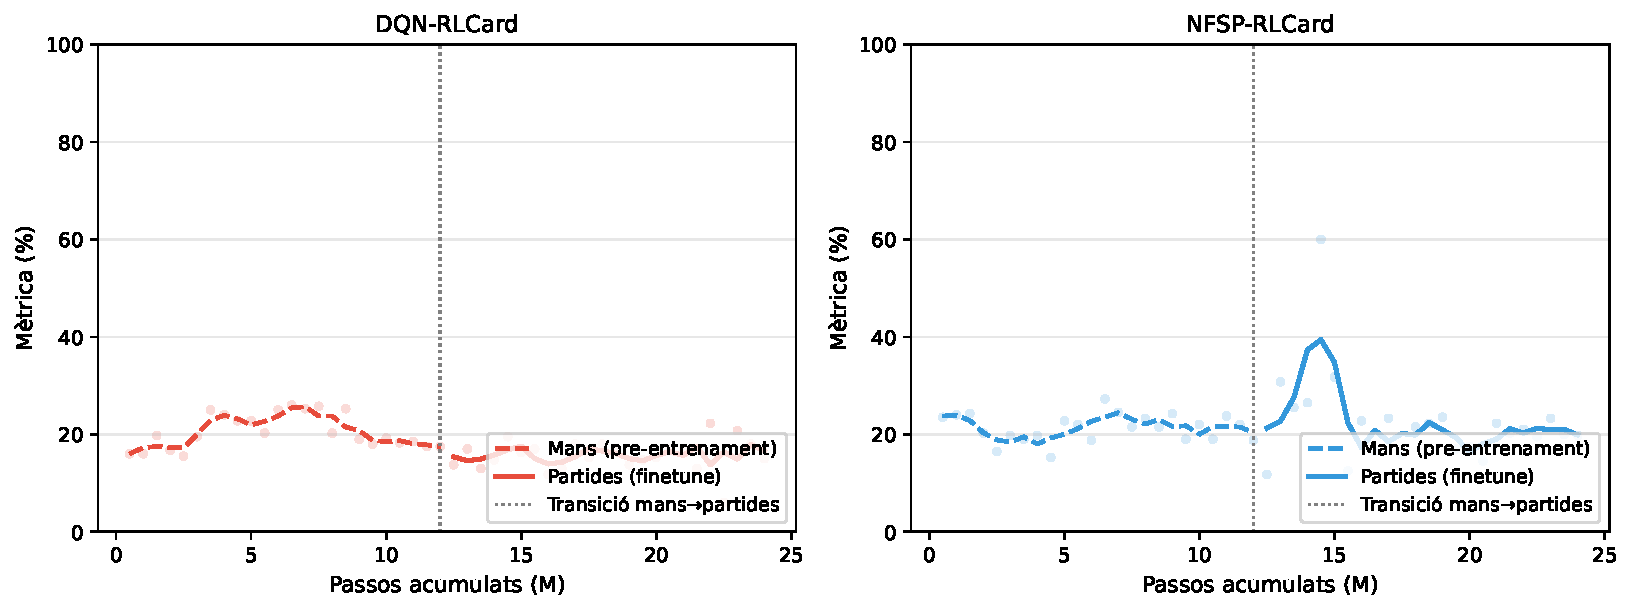
\includegraphics[width=\textwidth]{figures/fase2/curriculum_rlcard.pdf}
  \caption{Corbes del \emph{curriculum} per als agents RLCard. La línia ratllada
           és la fase de mans (pre-entrenament); la línia sòlida el \emph{finetune}
           sobre partides. La línia puntejada marca la transició als 12M passos.
           DQN-RLCard col·lapsa al \emph{finetune}; NFSP-RLCard recupera i millora
           lleugerament.}
  \label{fig:fase2-curriculum-rlcard}
\end{figure}

\begin{figure}[H]
  \centering
  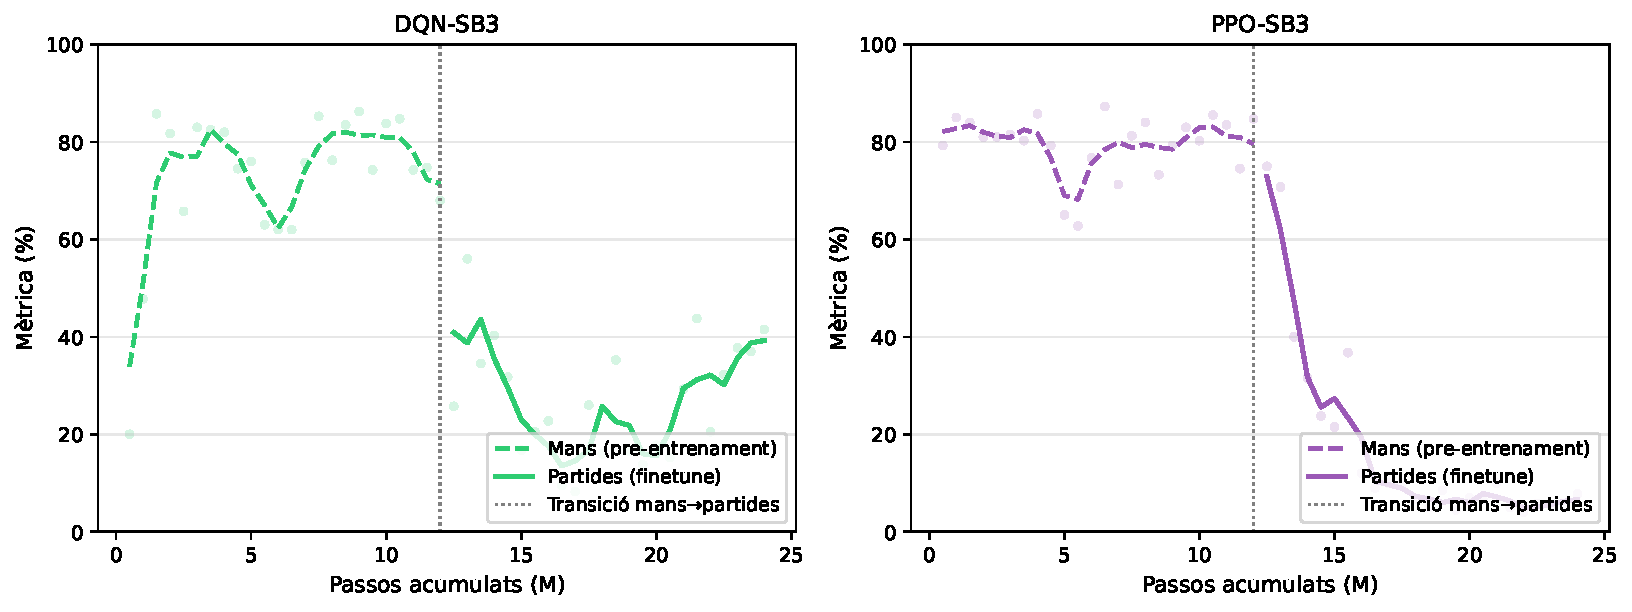
\includegraphics[width=\textwidth]{figures/fase2/curriculum_sb3.pdf}
  \caption{Corbes del \emph{curriculum} per als agents SB3. DQN-SB3 assoleix un pic
           alt en mans (86\%) però perd rendiment al \emph{finetune}. PPO-SB3 manté
           el nivell i tanca a 75\%, el millor resultat del treball fins al moment.}
  \label{fig:fase2-curriculum-sb3}
\end{figure}

El cas més destacat és \textbf{PPO-SB3}, l'agent més feble de la Fase~1: passa del 35\%
al 75\% amb el curriculum complet (+40~punts), el millor resultat del treball fins
aleshores. Es valida que el problema de PPO no era l'algorisme sinó l'horitzó llarg amb
recompensa diferida. En canvi, \textbf{DQN-RLCard} col·lapsa al \emph{finetune} (22{,}2\%):
la seva implementació no integra bé la càrrega de pesos previs i, sense el \emph{self-play}
regularitzador de la Fase~1, perd estabilitat.

\paragraph{Decisió.} El \emph{curriculum learning} millora el rendiment, però de manera
condicionada a l'agent: a igualtat de 12M passos tots quatre agents aprenen molt millor
sobre mans, però després del \emph{finetune} només PPO-SB3 (massivament) i NFSP-RLCard
(lleugerament) en surten beneficiats al pressupost total. El coll d'ampolla, doncs, és la
\textbf{transferència} de mans a partides, no l'aprenentatge inicial; i el curriculum
queda validat com a tècnica clau per a PPO-SB3.

\subsection{Checkpoint 1: models seleccionats}
\label{sec:checkpoint1}

Tancades les Fases~1 i~2, cal decidir quins dels quatre models continuen a la resta del
treball. El criteri combina el rendiment (\texttt{metric}) i el cost d'entrenament, i el
resultat és clar: avancen els dos agents \ac{SB3} i es descarten els dos de RLCard.

\textbf{PPO-SB3} és el gran beneficiari del curriculum i passa a ser el \emph{baseline} de
referència. Del 35\% puja al 75\% amb el curriculum complet (el millor resultat del treball
fins aleshores) i és el millor aprenent sobre mans (87,2\%), amb aproximadament la meitat
del cost de DQN-SB3 ($\sim$40~min davant de $\sim$5,5~h per execució). La seva narrativa
resumeix la lliçó del bloc: PPO no tenia un problema de capacitat sinó de senyal
d'aprenentatge, i el curriculum el resol. El seu \emph{throughput} excel·lent permet, a
més, iterar ràpidament a les fases següents. \textbf{DQN-SB3} es manté com a \emph{baseline}
robust: és el millor sobre partides sense curriculum (60,5\%), té un sostre del 86,2\% sobre
mans i representa la família dels algorismes basats en la funció de valor, el contrapunt
natural a PPO; el
seu cost ($\sim$5,5~h per execució) és assumible per als experiments llargs de les fases
següents.

Es descarten, en canvi, els dos agents de RLCard. \textbf{DQN-RLCard} pateix un oblit
catastròfic sever al \emph{finetune} (col·lapsa al 22\%) i és consistentment inferior a
DQN-SB3 en tots els experiments. \textbf{NFSP-RLCard} és l'algorisme més lent
($\sim$17~h per execució), no supera el 60\% de \texttt{metric} i no mostra cap
escalabilitat amb més còmput: el benefici és massa modest per al cost.
